The centralized server architecture represents a most principal component in the hybrid edge-server person Re-ID system, serving as the computational backbone for resource-intensive operations that exceed the capabilities of edge devices. While the CPU-based edge devices handle distributed object detection and initial preprocessing, the centralized server leverages its GPU computing resources to perform sophisticated model inference tasks, including feature extraction and gender classification. Additionally, the server manages vector database operations for identity storage and retrieval, coordinates multi-consumer message processing from Kafka streams, and maintains the overall system state for cross-camera identity matching, as illustrated in Figure \ref{fig:centralized_server_overview}. This centralized microservice-based approach enables the system to achieve optimal resource utilization by offloading computationally demanding tasks from resource-constrained edge devices to a dedicated server environment equipped with specialized hardware acceleration. The server's architecture is designed to handle concurrent processing of multiple video streams while maintaining real-time performance requirements essential for practical surveillance applications.

\newpage
\begin{figure}[!htbp]
    \centering
    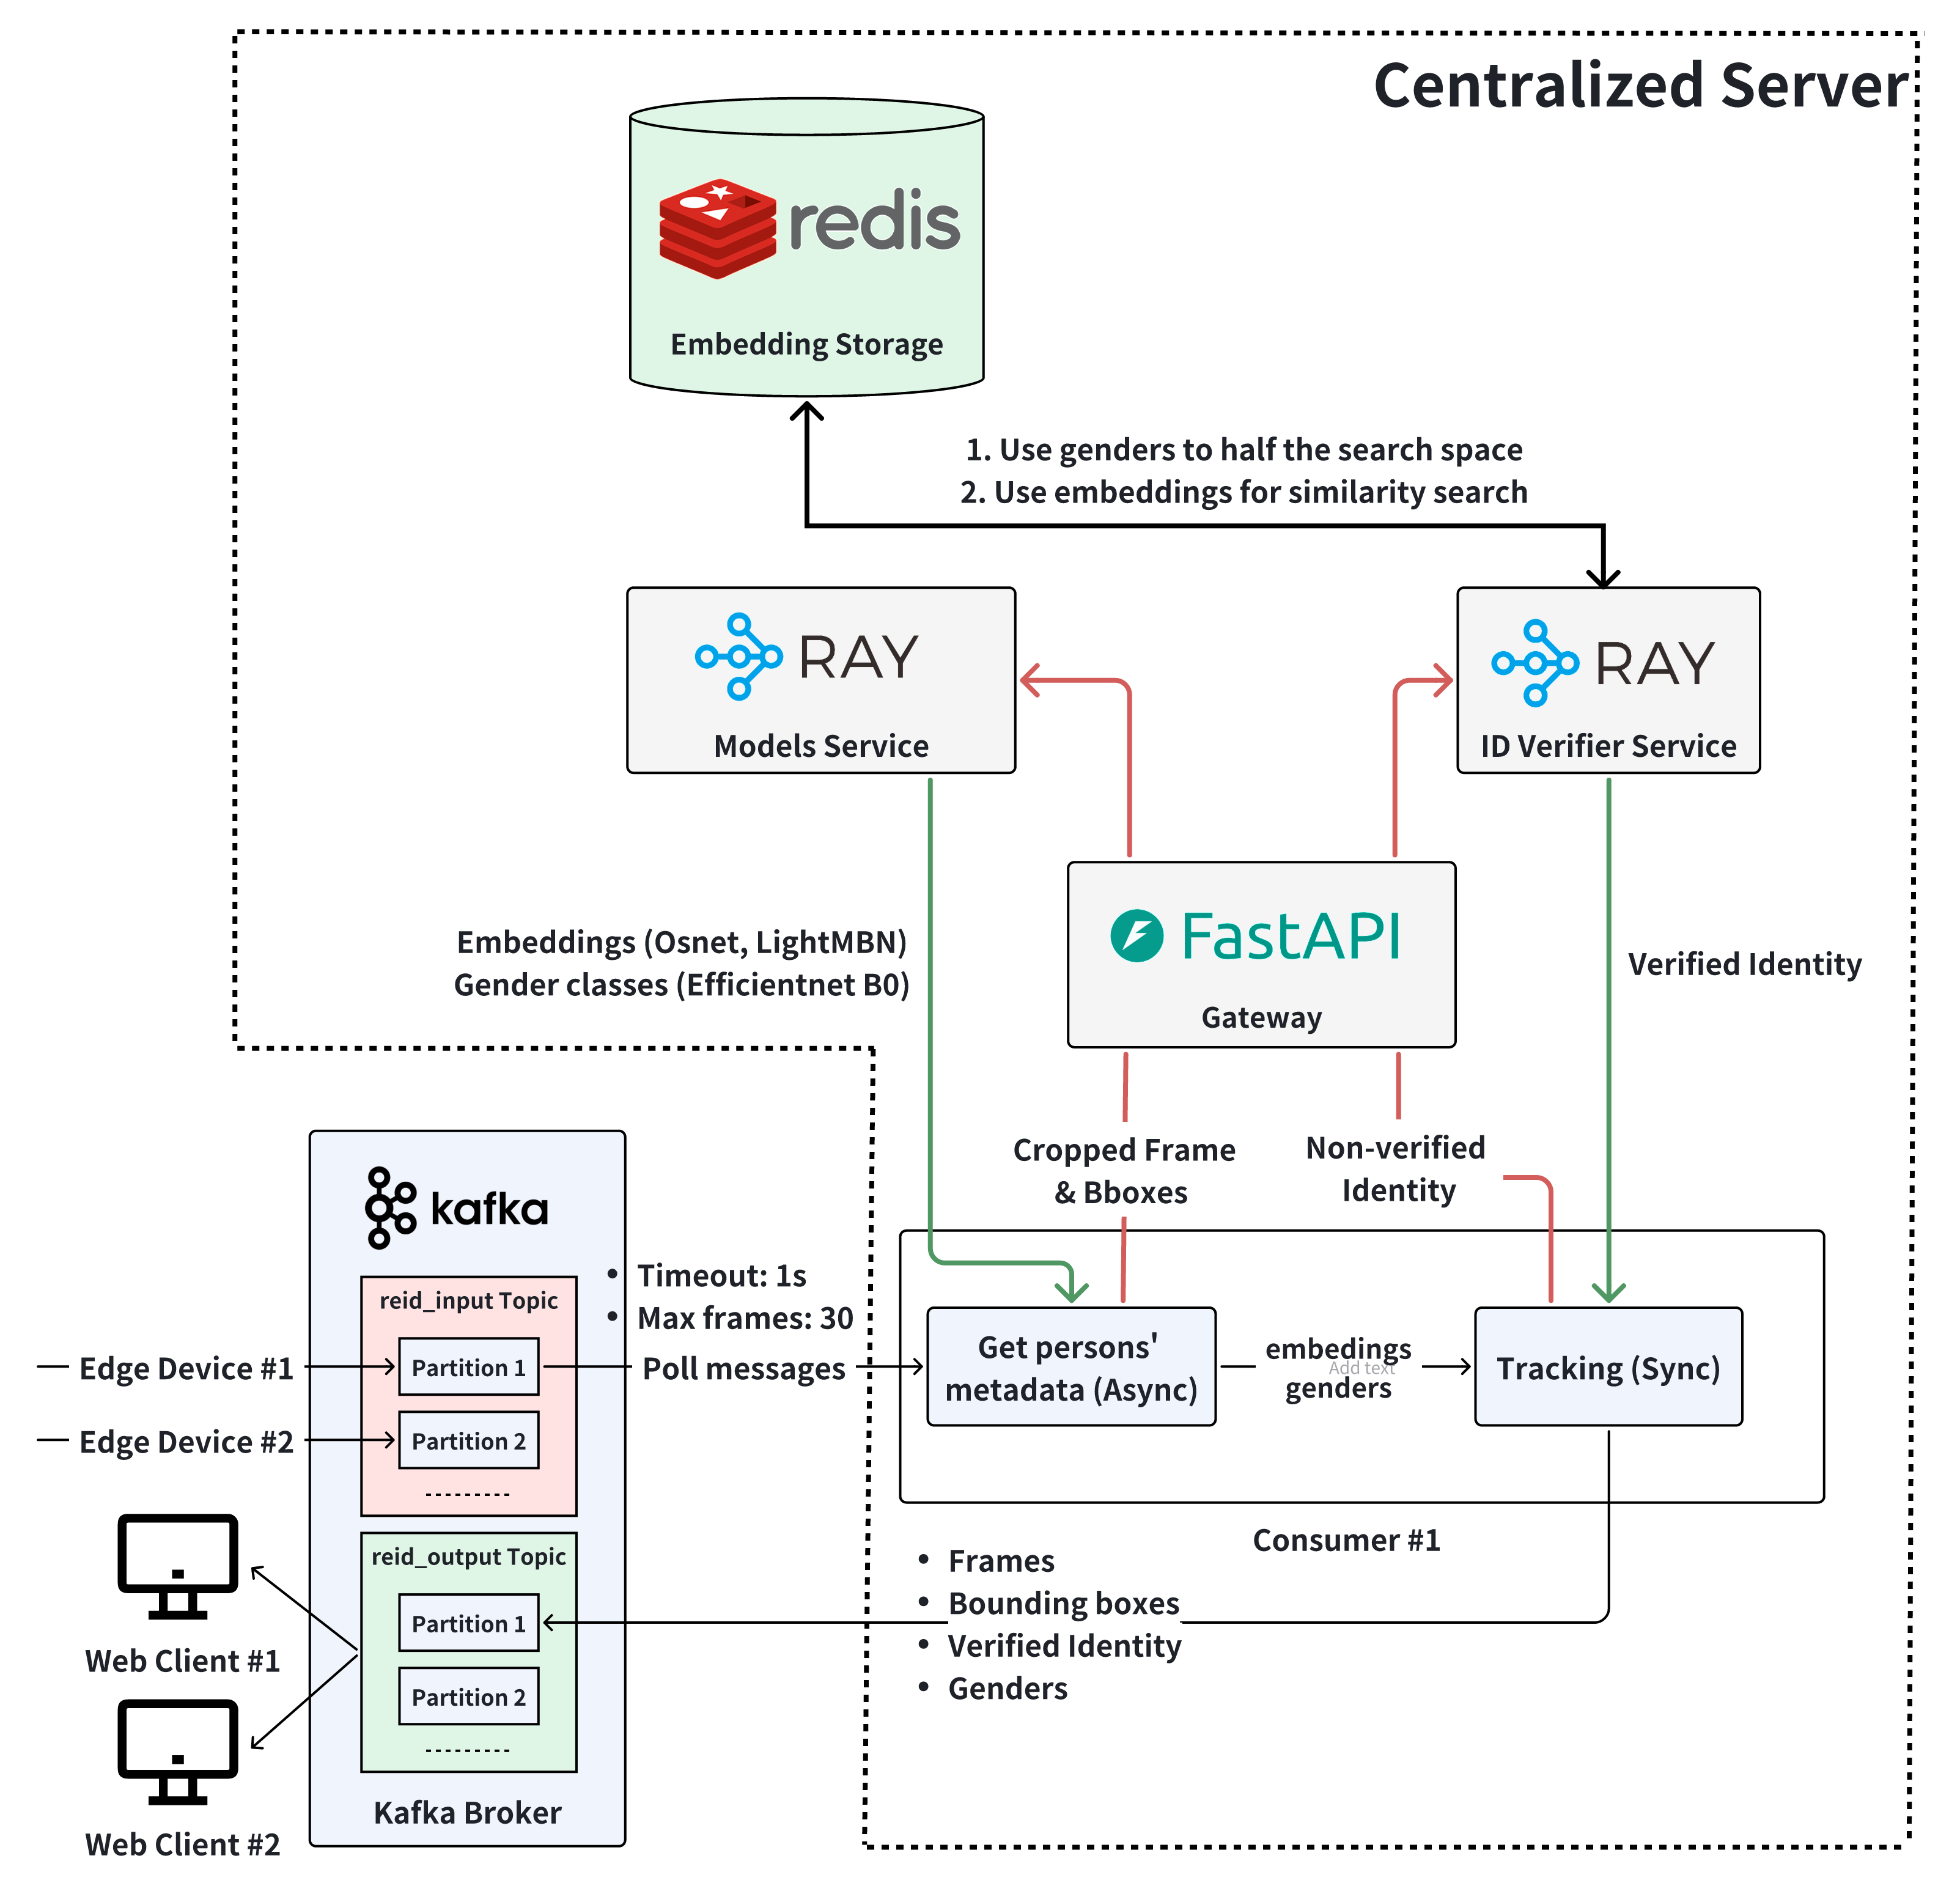
\includegraphics[width=1.1\textwidth]{Figure/centralized_overview.png}
    \caption{Centralized server architecture. The server is equipped with a decent GPU and CPU, and it is responsible for performing sophisticated model inference tasks, vector database operations, and multi-consumer message processing.}
    \label{fig:centralized_server_overview}
\end{figure}

\subsection{System Data Flow and Processing Pipeline}

The centralized server architecture orchestrates a complex data flow that transforms raw video streams into actionable identity verification results through multiple interconnected services. As depicted in Figure \ref{fig:centralized_server_overview}, the processing pipeline begins when edge devices capture and preprocess video frames, transmitting video frames, cropped person detections, and bounding box coordinates through Kafka message queues to the centralized server.

Each partition of the Kafka topics corresponds to a specific camera feed, and each consumer group is responsible for processing messages from a single partition, ensuring that message ordering is preserved—a critical requirement for the tracking module of the Re-ID system. As illustrated in Figure \ref{fig:centralized_server_overview}, Consumer \#1 represents the data processing pipeline that serves as a template for additional consumers. Each consumer operates within an event loop that fetches batched messages (maximum 30 messages) from its assigned Kafka topic partition every 1 second. This batched processing approach significantly reduces computational overhead compared to continuous message fetching, while maintaining near real-time processing capabilities essential for surveillance applications.

After receiving the batch of messages, the system processes each message (frame) through a structured pipeline:

\begin{enumerate}
   \item For each frame containing cropped person detections and bounding box coordinates, the system extracts person regions and computes two essential properties (referred to as \textbf{person metadata}):
   \begin{itemize}
       \item \textbf{Embedding vector}: A numerical feature representation of the person region used for similarity searches in the vector database to determine whether the person already exists in the system.
       \item \textbf{Gender classification}: The predicted gender of the person (male or female), enabling gender-based search space partitioning that reduces computational complexity by approximately 50\% by querying only relevant gender subsets during similarity matching operations.
   \end{itemize}
   \item The processing goal is to obtain complete results for all frames in the batch before proceeding to tracking and identity matching operations.
\end{enumerate}

The first processing step does not require maintaining frame order, as the primary objective is achieving accurate and efficient results that can be sorted by timestamp before performing tracking and identity matching. This independence from sequential processing makes asynchronous processing an optimal approach for the initial metadata extraction phase, allowing parallel computation of embeddings and gender classifications across multiple frames simultaneously to maximize throughput and minimize processing latency.


\subsubsection{Message Processing using Ray Serve through FastAPI Gateway}

\begin{enumerate}
    \item \textbf{FastAPI Gateway}\\
    
    The \textbf{FastAPI Gateway} acts as the central coordination layer that orchestrates the processing pipeline between Kafka consumers and Ray Serve services. As depicted in Figure \ref{fig:centralized_server_overview}, when consumers poll batched messages (cropped frames and bounding boxes) from their assigned Kafka partitions, the processing follows a sequential workflow via the FastAPI Gateway. First, the \textbf{Get person's metadata (Async)} module sends all cropped frames in the batch to the RAY Models Service for feature extraction (Osnet, LightMBN embeddings) and gender classification (EfficientNet B0). After all frames in the batch are processed, the results are sorted by their original timestamps to maintain temporal order before proceeding to the tracking phase.

    The sorted embeddings and gender classifications are then forwarded to the customized \textbf{Tracking (Sync)} module, which iterates through each frame in correct timestamp order. The tracking module (ByteTrack or BOTSort) uses detection results and embeddings to perform association with previous tracklets, returning a list of person IDs for each frame. Crucially, only newly discovered IDs that do not exist in previous tracklets are considered "non-verified" and require database verification. This is because tracking algorithms can only maintain ID persistence in the short term and cannot determine whether a person actually existed in the system previously.

    For these non-verified IDs, the tracking module requests the RAY ID Verifier Service to query the Qdrant vector database using gender-based search space partitioning and embedding similarity search. Once verified identities are returned, the tracking module updates its tracklet data with the correct IDs, ensuring that subsequent frames do not require repeated database queries for the same person, as the tracking module only consults the ID verifier service when encountering new, unrecognized identities.

    \item \textbf{Models Service}\\

    The \textbf{Models Service} is wrapped by Ray Serve framework, responsible for performing dual-model inference operations, executing either \textbf{OSnet} or \textbf{LightMBN} for robust feature extraction, while still able to run \textbf{EfficientNet B0} simultaneously for gender classification. This parallel inference approach maximizes GPU utilization while providing complementary identity features that enhance matching accuracy across diverse scenarios.

    \item \textbf{ID Verifier Service}\\
    
    
\end{enumerate}



\textbf{Models Service Processing}: The RAY Models Service performs dual-model inference operations, executing both Osnet and LightMBN architectures for robust feature extraction, while simultaneously running EfficientNet B0 for gender classification. This parallel inference approach maximizes GPU utilization while providing complementary identity features that enhance matching accuracy across diverse scenarios.

\textbf{Identity Verification Workflow}: Extracted embeddings are forwarded to the RAY ID Verifier Service, which interfaces with the Qdrant vector database to perform similarity searches against stored identity profiles. The service employs gender-based search space partitioning to reduce computational complexity by approximately 50\%, querying only relevant gender subsets during similarity matching operations.

\textbf{Asynchronous Metadata Retrieval}: The system implements asynchronous metadata retrieval to optimize processing throughput, where person metadata (including historical profiles, timestamps, and camera associations) is fetched concurrently with embedding computation, minimizing end-to-end latency.

\subsubsection{Multi-Consumer Architecture and Load Distribution}

The Kafka-based messaging system implements a partitioned topic structure that enables horizontal scaling across multiple edge devices. Each partition corresponds to individual camera feeds, allowing the centralized server to process multiple video streams simultaneously without cross-contamination. The Consumer \#1 component demonstrates the scalable consumer group pattern, where additional consumers can be dynamically instantiated to handle increased throughput demands.

The tracking synchronization module maintains temporal consistency across the distributed system, correlating detection events with their corresponding metadata and ensuring that identity verification results are properly associated with their originating video streams and timestamps.

\subsubsection{Output Distribution and Client Integration}

Processed results, including verified identities, gender classifications, bounding box coordinates, and confidence scores, are published back to Kafka output topics using the same partitioned structure. This bidirectional communication pattern enables multiple web clients to subscribe to specific camera feeds or system-wide notifications, supporting diverse use cases from real-time monitoring dashboards to forensic analysis applications.

The architecture's microservice design ensures fault tolerance and independent scaling, where individual services can be replicated or upgraded without affecting the overall system operation, making it suitable for production deployment in enterprise surveillance environments.


\subsection{Models service}

    \subsubsection{Ray Serve configuration}

    \subsubsection{Feature extraction}

    \subsubsection{Gender classification}

\subsection{Vector database service}

    \subsubsection{Qdrant configuration}

    \subsubsection{Identity embedding storage}

    \subsubsection{Identity retrieval}

\subsection{Consumers}